\chapter{Objetivos}
\title{Objetivos}

\title{Objetivos principales}
\section{
Objetivos principales
}
Se desea desarrollar un \textbf{sistema que permita sincronizar a los músicos de una banda} entre sí,
utilizando \textbf{tecnologías libres}. Debido al número de horas que puede llegar a durar una
actuación, se quiere que tenga un \textbf{bajo consumo energético} (y conseguir que la vida de la batería se alargue).
También se quiere que sea
\textbf{vestible}, de forma que sea cómodo y discreto para el usuario. Por supuesto, para que
sea competitivo, debe ser \textbf{más barato que otras soluciones} disponibles en el mercado y
\textbf{escalable en el número de dispositivos}. Se pretente, además, que sea \textbf{posible añadir nuevas
funciones a posteriori}.\\

Se desea utilizar tecnologías libres para que cualquier desarrollador pueda aportar su conocimiento al proyecto, colaborando
con aquellas bandas de música que utilicen el producto. Además, como ya se dijo en la introducción,
una comunidad alrededor de este producto podría mejorar el rendimiento del mismo y añadir nuevas funcionalidades.\\

El hecho de que el sistema sea vestible viene por dos razones: comodidad (los músicos llevarían mucho tiempo encima el aparato y,
unido al instrumento y partituras, un dispositivo que sea demasiado grande, será un lastre) y decoro (no queda bien de cara al público que
un músico vestido de gala lleve un aparato que sea demasiado llamativo).\\

La sincronización que se pretende llevar a cabo es la solución al problema planteado durante la introducción: es complicado
mantener acompasados a todos los músicos de una banda mientras se está realizando una actuación en la calle y el director no puede
realizar adecuadamente sus funciones.\\

Los objetivos no se encuentran muy interconectados. El bajo consumo energético y que sea vestible se encuentran
relacionados (si tiene un consumo energético muy alto, se pasará más tiempo dependiendo de la conexión a una fuente
de alimentación no portable del que debiera). Por otro lado, al querer construir un sistema que permita comunicación,
será necesario que sea escalable (cuanta más escalabilidad permita, mayor será el número de personas que podamos conectar).

Todos los objetivos se tratan durante el capítulo 7 (correspondiente a la implementación del sistema) excepto
la creación de un dispositivo más barato que otros productos del mercado (se hablará de esto en los capítulos 4 -cuando se
estimen costes- y en el capítulo 8 -donde se comparará con otro sistema existente en el mercado-) y la posibilidad de añadir
nuevas funciones (que se tratará en el capítulo 8).


\title{Consideraciones técnicas}
\section{Consideraciones técnicas}

  \begin{itemize}
    \item Una posible solución al problema planteado puede ser el despliegue de una red inalámbrica de sensores,
    más teniendo en cuenta la actual dirección de la industria respecto a este tipo de tecnología (su aplicación,
    por ejemplo en el “Internet de las Cosas”, que se encuentra en la cima de la curva de Gartner \ref{fig:curvaG})
    \item La creación de dispositivos \textit{wearables} es algo que también ha suscitado
    mucha atención por parte de la industria (como también se puede ver en la curva de Gartner)
  \end{itemize}

  \begin{figure}[htb]
  \centering
  \captionsetup{justification=centering}
  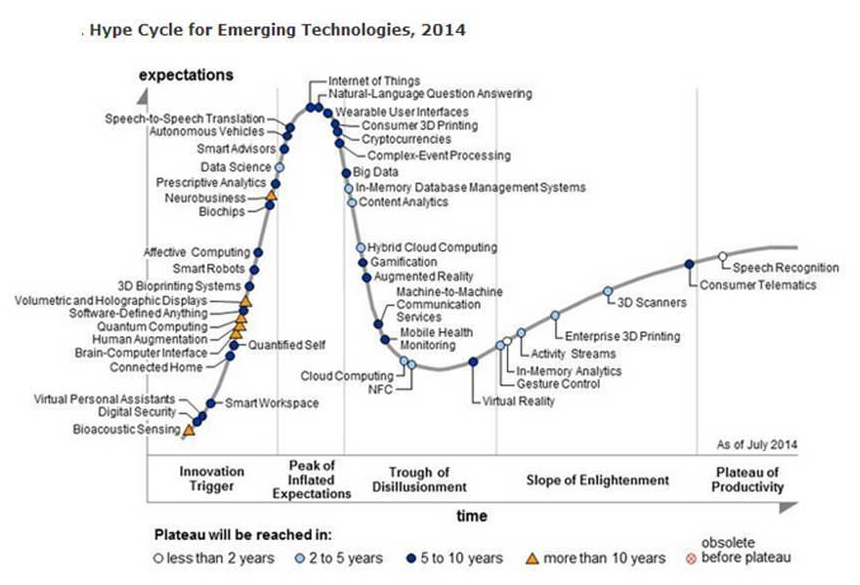
\includegraphics[width=1\textwidth]{./imagenes/gartner}
  \caption{Curva de Gartner (agosto de 2014)\\
    \scriptsize{Imagen extraída de http://www.gartner.com/}
  \cite{gartnercurve}} \label{fig:curvaG}
  \end{figure}

La Gartner es una empresa consultora especializada en nuevas tecnologías. La curva de Gartner es
un estudio realizado por esta empresa en el que se analizan distintas tecnologias
y su estado en el momento de la investigación (fase de lanzamiento, pico
de altas expectativas, valle de la desilusión, rampa de la consolidación o meseta
de la productividad).\\

\title{Aspectos formativos previos}
\section{Aspectos formativos previos}

Aunque todo el conocimiento obtenido durante el grado ha sido importante para el desarrollo del proyecto, hay que destacar:
  \begin{itemize}
    \item Fundamentos de Ingeniería del Software: para establecer los requisitos,
    la planificación, costes de desarrollo...
    \item Programación de Dispositivos Móviles: para realizar las aplicaciones ``Android"
    \item Tecnologías Emergentes: en esta asignatura se ha impartido materia sobre el uso
    de placas controladoras, dispositivos \textit{wearables} y redes inalámbricas de sensores
    \item Informática Industrial: algunos conocimientos sobre redes inalámbricas de sensores
    \item Fundamentos de Redes: para comprender las distintas capas de los protocolos analizados y
    la estructura de los paquetes que se envían entre sí los dispositivos
  \end{itemize}
